\documentclass[preprint,review,12pt,authoryear]{elsarticle}
\usepackage{amsmath,amssymb,amsthm}
\usepackage{booktabs}
\usepackage{graphicx}
\usepackage{xcolor}
\usepackage{algorithm}
\usepackage{algpseudocode}
\usepackage{adjustbox}
\usepackage{tikz}
\usepackage[hidelinks]{hyperref}

\newtheorem{theorem}{Theorem}
\newtheorem{proposition}[theorem]{Proposition}
\newtheorem{corollary}[theorem]{Corollary}
\newtheorem{assumption}{Assumption}
\theoremstyle{definition}
\newtheorem{definition}{Definition}
\newtheorem{remark}{Remark}

\newcommand{\E}{\mathbb{E}}
\newcommand{\Var}{\operatorname{Var}}
\newcommand{\diag}{\operatorname{diag}}
\newcommand{\tW}{\tilde W}
\newcommand{\tY}{\tilde Y}
\setlength{\emergencystretch}{3em}

\journal{Information Processing \& Management}

\begin{document}
\begin{frontmatter}

\title{Causal graph recommendation under exposure bias: removing the repeated-walk bias of doubly robust propagation}

% Anonymised for double-anonymised review: author details are given on the
% separate title page (title_page.tex).

\begin{abstract}
Graph recommenders trained on logged data propagate preferences along walks that can traverse an edge more than once. With inverse-propensity or doubly robust (DR) edge estimates, such walks multiply an estimate with itself and bias multi-hop scores. We derive this bias exactly and remove it with DRUP, an idempotent walk correction that is exact for any odd number of hops and costs about as much as the uncorrected three-hop operator. We test it on Coat, Yahoo! R3, KuaiRand and KuaiRec (290 to 15,400 users; up to 10.3 million logged interactions) against up to 26 tuned baselines, and on a semi-synthetic KuaiRec log with known exposure. With true propensities and fixed weights, the correction reduces the error of the three-hop term by a factor of 4 to 12 and removes an 18--29\% overestimate of an allocation's utility; with estimated propensities, all operators overstate utility by 100--540\%. Accuracy does not change: corrected and uncorrected three-hop DR propagation differ by at most 0.0014 nDCG. The guarantees need nuisances independent of the log: with degree weights computed from the log the correction no longer reduces bias, and the sample-split variant that satisfies them loses up to 0.06 nDCG on sparse logs. On KuaiRec, training-free DR propagation (nDCG@20 0.638) leads the best trained model by 0.004, within that model's seed spread.
\end{abstract}

\begin{keyword}
Causal recommendation \sep causal graph recommendation \sep doubly robust estimation \sep exposure bias \sep missing not at random \sep graph-based recommendation \sep exposure invariance.


%======================================================================
\end{keyword}

\end{frontmatter}

\section{Introduction}
%======================================================================

Graph-based recommenders represent users and items as nodes and logged
interactions as edges, and they score a user--item pair by aggregating signals
along multi-hop walks~\citep{he2020lightgcn,shen2021gfcf}. The logged graph is
not the preference graph. An edge exists only if the platform \emph{exposed}
the item and the user then responded, so the graph records the exposure policy
as much as the user's taste. Causal learning offers two families of
corrections. \emph{Loss-level} debiasing re-weights the training objective by
inverse propensities or doubly robust (DR)
terms~\citep{schnabel2016,wang2019drjl,saito2020unbiased}, but it leaves the
propagation operator of a graph model untouched. \emph{Propagation-level}
debiasing changes the propagated graph, for example by weighting each edge by
its inverse propensity~\citep{kim2022navip} or by learning popularity-aware
aggregation weights~\citep{zhou2023apda,dpaa2026}.

This paper starts from a simple observation about the second family. An
inverse-propensity edge estimate $W_e=O_eY_e/p_e$ is unbiased for the potential
outcome $Y_e$, where $O_e$ indicates that edge $e$ was exposed, $Y_e$ is the
outcome and $p_e$ the exposure propensity. A walk that traverses $e$ twice
contributes $W_e^2$, and $\E[W_e^2]=Y_e/p_e\neq Y_e$. The same holds for DR edge
estimates. Walks that repeat an edge are part of every multi-hop operator: the
back-and-forth step $u\to j\to u$ of a three-hop walk is one. Their excess is
largest where the propensity is smallest, that is, on the rarely exposed edges
that debiasing is meant to recover.

%======================================================================
\section{Research objectives and contributions}\label{sec:objectives}
%======================================================================

The aim of this study is to determine whether and when removing the
repeated-walk bias helps graph recommendation from exposure-biased logs. We
pursue four objectives, each tied to a research question (RQ).

\begin{description}
\item[O1 (estimator).] Derive the exact bias of inverse-propensity and DR graph
propagation and an estimator that removes it. \emph{RQ1: how large is the bias,
and can it be removed exactly at a cost comparable to the uncorrected operator?}
\item[O2 (conditions).] State the conditions under which the correction is
unbiased and test them in the way practitioners fit nuisances. \emph{RQ2: do the
guarantees survive cross-fitting and data-dependent degree weights?}
\item[O3 (value).] Measure what the correction changes. \emph{RQ3: does it
improve the accuracy of recommendations against tuned baselines on four
benchmarks, and does it improve the values of the scores on a log with known
exposure?}
\item[O4 (invariance).] Test on real logs the prediction that expected scores do
not depend on an item's exposure. \emph{RQ4: how informative is a thinning audit
of this property?}
\end{description}

\paragraph{Answers in brief} The bias is exact and removable at three hops for
the cost of one item Gram matrix (RQ1). The guarantees need nuisances that do
not depend on the log: cross-fitting suffices if the degree weights are fixed a
priori, but not if they are computed from the log, which our experiments do
(RQ2). The correction leaves accuracy unchanged on four datasets, and it
improves score values only under oracle conditions: true propensities and
weights fixed in advance (RQ3). The thinning audit has little power and the
selected configurations are not invariant on two of four datasets (RQ4).

\paragraph{Contributions}
\begin{enumerate}
\item \emph{Diagnosis.} The exact conditional bias of inverse-propensity and DR
propagation on unexposed candidates; under a propensity clip $\tau$ its worst
case is $\Theta(1/\tau)$ (Theorem~\ref{thm:lower}).
\item \emph{Estimator.} DRUP (Doubly Robust, walk-Unbiased Propagation) uses
$Y_e^2=Y_e$ for binary outcomes and replaces each repeated edge by its
idempotent unbiased counterpart. The three-hop operator has the asymptotic cost
of the uncorrected one, and Möbius inversion over the coincidence patterns of
walk indices makes the correction exact for any odd number of hops
(Theorem~\ref{thm:khop}). A sample split supplies nuisances independent of the
edge estimates (DRUP-split).
\item \emph{Guarantees and their scope.} With nuisances independent of the log,
DRUP is edge-wise doubly robust for propagation over the full-exposure graph
(Theorem~\ref{thm:unbiased}), unbiased on unexposed candidates up to the
imputation error at the candidate (Corollary~\ref{cor:cand}), and its expected
scores do not respond to interventions on an item's exposure
(Theorem~\ref{thm:fair}). We show by simulation where these guarantees fail.
\item \emph{Evidence.} A semi-synthetic test on KuaiRec with known exposure;
a comparison with up to 26 tuned baselines on Coat, Yahoo!\,R3, KuaiRand and
KuaiRec with user-level tests; and real-data thinning audits with a negative
control. The properties that follow from linearity alone (attributions,
certificates, private release, capped allocation) are in the Supplementary
Material.
\end{enumerate}

\paragraph{Outline} Section~\ref{sec:related} reviews related work,
Section~\ref{sec:drup} presents the method, Section~\ref{sec:setup} the datasets,
baselines and protocol, Section~\ref{sec:results} the results, and
Section~\ref{sec:disc} the theoretical and practical implications and limits.

%======================================================================
\section{Related work}\label{sec:related}
%======================================================================

\paragraph{Graph-based recommendation}
Graph neural recommenders propagate embeddings over the user--item graph.
LightGCN~\citep{he2020lightgcn} removes feature transformations and
non-linearities, which reduces propagation to a weighted sum of powers of a
normalised adjacency; UltraGCN~\citep{mao2021ultragcn} approximates
infinite-layer propagation, and SGL~\citep{wu2021sgl} and
SimGCL~\citep{yu2022simgcl} add contrastive views. Closed-form models are strong
competitors: EASE~\citep{steck2019ease} and EDLAE~\citep{steck2020edlae} learn an
item--item matrix with a constrained diagonal, which, like our diagonal
correction, removes an item's own contribution to its score;
GF-CF~\citep{shen2021gfcf} and BSPM~\citep{choi2023bspm} cast collaborative
filtering as graph signal filtering. Carefully tuned simple baselines often
match graph models~\citep{anelli2023myth}. All of these propagate over the
\emph{logged} graph. DRUP keeps the linear propagation form but propagates over
an unbiased estimate of the full-exposure graph.

\paragraph{Debiasing in recommendation}
Logs are missing not at random~\citep{marlin2009collaborative}; surveys organise
the resulting biases and cast debiasing as causal
inference~\citep{chen2023bias,gao2024causalsurvey}. Propensity-based methods
re-weight the loss~\citep{schnabel2016,swaminathan2015snips,saito2020unbiased}.
Doubly robust learning adds an imputation model~\citep{wang2019drjl}, and later
variants reduce its bias and variance~\citep{guo2021mrdr,dai2022gdr,li2023stabledr}.
A small uniform sample can supervise the debiasing~\citep{chen2021autodebias}.
Causal approaches to popularity bias use counterfactual
inference~\citep{wei2021macr}, confounder adjustment~\citep{zhang2021pda} or
disentangled representations~\citep{zheng2021dice}; recent work in this journal
studies popularity debiasing from both sides~\citep{boratto2021connecting}, with a
controllable trade-off~\citep{okamura2024flexibly}, through invariant
learning~\citep{bai2025invariant} and through causal deconfounding of
multi-criteria ratings~\citep{guo2026confounding}. These methods correct the loss
or the output of a model; DRUP applies inverse-propensity and DR estimation to the
\emph{edges} of the propagated graph.

\paragraph{Debiasing inside graph propagation}
NAVIP~\citep{kim2022navip} weights each edge by its inverse propensity inside
LightGCN. r-AdjNorm~\citep{zhao2022radjnorm} tunes the adjacency normalisation
that controls the amplification of popularity, and graph convolutions provably
amplify popularity bias~\citep{chen2024gcnpop}. APDA~\citep{zhou2023apda},
CAGED~\citep{que2025caged} and DPAA~\citep{dpaa2026} learn aggregation weights.
These methods change \emph{which} adjacency is propagated. None analyses what
happens to an unbiased edge estimate when the re-weighted adjacency is multiplied
with itself over several hops. Theorem~\ref{thm:lower} shows that the product is
then biased by a term of order $1/p$ that concentrates on rarely exposed items.
Our linear baseline over the logged graph searches the normalisation exponent and
is therefore a training-free r-AdjNorm; we also train r-AdjNorm and NAVIP.

\paragraph{Unbiased estimation of polynomials under missingness}
An unbiased estimator of a polynomial in unknown quantities must avoid products of
the same noisy measurement, as in U-statistics~\citep{hoeffding1948}. For
Bernoulli-masked data the masked Gram matrix needs a $1/p^2$ correction off the
diagonal and $1/p$ on it~\citep{lounici2014}; our item operator is the analogue
with heterogeneous propensities. Möbius inversion on the partition
lattice~\citep{rota1964} turns homomorphism counts into injective counts and is
the combinatorial counterpart of our $K$-hop construction. Non-backtracking
operators~\citep{krzakala2013} and self-avoiding walks~\citep{hopkins2017bayesian}
discard repeated walks; our correction keeps them and replaces each repeated
factor by its unbiased counterpart. In recommendation,
\citet{schnabel2020item} debias item co-occurrence with propensities. The
reduction itself is therefore not new; what is new is its combination with
inverse-propensity and DR edge estimates and degree weights, the exact bias of the
uncorrected operators, and the consequences for exposure invariance. Our
treatment of nuisances follows double machine learning~\citep{chernozhukov2018dml}.

\paragraph{Fairness, explanation, robustness and privacy}
Fairness notions cover users and items, groups and individuals, and outcomes and
exposure~\citep{wang2023fairness,amigo2023fairness}; item-side exposure can be
allocated in proportion to merit~\citep{singh2018exposure,diaz2020expected}, and
multi-stakeholder views weigh users, providers and the
platform~\citep{abdollahpouri2020multistakeholder,ekstrand2022fairness}. DRUP
contributes a causal property of the merit \emph{estimate}, exposure invariance,
which is not a fairness criterion. Graph explainers search for important or
minimal edge sets~\citep{ying2019gnnexplainer,lucic2022cfgnn,ghazimatin2020prince},
recommenders can be attacked by injected
profiles~\citep{lam2004shilling,li2016poisoning,fang2018poisoning}, and private
recommenders perturb statistics or matrix
completion~\citep{mcsherry2009netflix,jain2018dpmc}. Any linear operator with fixed
nuisances admits exact removal attributions, closed-form certificates and a jointly
private release of its item operator~\citep{balle2018analytic,hsu2014matchings};
these are in the Supplementary Material.

\begin{table}[t]\centering\footnotesize
\caption{DRUP and representative related methods. ``loss'': the correction
acts on the training objective; ``output'': it acts on the predictions;
``learned'': learned aggregation weights; ``--'': not applicable. Properties
that follow from linearity (exact attributions, certificates, joint DP) hold
for every linear operator, including linear LightGCN, GF-CF and DR adjacency,
and are not listed.}\label{tab:related}
\setlength{\tabcolsep}{4pt}
\begin{adjustbox}{max width=\textwidth}
\begin{tabular}{lcccc}
\toprule
Method & \shortstack{debiases\\propagation} & \shortstack{unbiased\\beyond 1 hop} & \shortstack{doubly\\robust} &
\shortstack{exposure\\invariance}\\
\midrule
\shortstack[l]{LightGCN, NGCF,\\UltraGCN, SGL, SimGCL} & no & no & no & no\\[2pt]
\shortstack[l]{linear LightGCN,\\EASE, GF-CF, BSPM} & no & no & no & no\\[2pt]
\shortstack[l]{IPS, SNIPS, DR,\\MRDR, StableDR} & loss & -- & DR variants & no\\[2pt]
MACR, PDA, DICE & output & -- & no & no\\
NAVIP & edge weights & no & no & no\\
\shortstack[l]{r-AdjNorm, APDA,\\CAGED, DPAA} & learned & no & no & no\\[2pt]
DR adjacency (uncorrected) & DR edges & no & edge-wise & no$^\ast$\\
\midrule
DRUP-split (ours; assumptions hold) & DR edges & any odd $K$ & yes$^\dagger$ & in expectation$^\dagger$\\
DRUP, cross-fitted (ours; as run) & DR edges & no$^\ddagger$ & no$^\ddagger$ & no$^\ddagger$\\
\bottomrule
\end{tabular}
\end{adjustbox}
\par\smallskip
\raggedright\scriptsize $^\ast$Over-corrects (Theorem~\ref{thm:fair}) with nuisances independent of the log; as invariant as DRUP in our real-data audits, which cannot tell them apart.
$^\dagger$Guaranteed under Assumptions~\ref{as:unconf}--\ref{as:fixed} (the sample split) and unclipped propensities.
$^\ddagger$No guarantee: nuisances are cross-fitted on the same log and degree weights and score constants are computed from it
(Remark~\ref{rem:xfit}); in simulation the correction then no longer reduces bias, and the audited configurations are not invariant on Yahoo!\,R3 and KuaiRand.
The cross-fitted operator is what the accuracy tables report; its accuracy equals that of uncorrected DR adjacency.
\end{table}

%======================================================================
\section{Problem setting}
%======================================================================

Users $u\in[m]$, items $i\in[n]$ and pairs $e=(u,i)$ carry a binary potential
outcome $Y_e\in\{0,1\}$ (whether $u$ would like $i$ if it were shown) and an
observation indicator $O_e\in\{0,1\}$. The log reveals $O$ and $O\odot Y$. What
$O$ records depends on the platform. On KuaiRec it is an impression chosen by
the system. On Coat and Yahoo!\,R3 it is a rating that the user chose to give,
so the ``exposure'' mechanism modelled by $p$ is then user self-selection
rather than the platform's display policy. All statements below are relative
to the mechanism that generates $O$. We keep the word exposure for brevity.

\begin{assumption}[Conditionally independent exposure]\label{as:unconf}
Conditionally on $Y$, the exposures $O_e$ are independent Bernoulli variables
with propensities $p_e=\Pr(O_e=1\mid Y)>0$.
\end{assumption}
The propensity may depend on the pair's own outcome, so the log may be missing
not at random. All expectations below are over $O$ given $Y$.

\begin{assumption}[Fixed nuisances]\label{as:fixed}
The propensity estimates $\hat p$, the imputation $\hat Y\in[0,1]^{m\times n}$,
the edge weights $C$ and the constants $a,b$ of the score below are fixed
given $Y$, i.e., they do not depend on $O$ (for instance, they are fitted on
an independent log). We use $C_{ui}=d_u^{-\alpha}d_i^{-(1-\alpha)}$ with degrees
$d$ taken from $\hat Y$.
\end{assumption}
The weights $C$ also enter the target below. With degrees from $\hat Y$, the
target therefore depends on the imputation. A normalisation fixed a priori (a
design choice, or degrees from an independent source) makes the target
independent of $\hat Y$; Section~\ref{sec:semisynth} compares both.

\begin{remark}[Scope of the guarantees and the experimental protocol]\label{rem:xfit}
All guarantees below are stated under Assumption~\ref{as:fixed}. Our main
experimental protocol does not satisfy it, in four ways. (i) $\hat p$ and
$\hat Y$ are cross-fitted over ten random folds of pairs: the nuisances used at
a pair of fold $k$ are fitted on the other nine
folds~\citep{chernozhukov2018dml}. This makes the nuisance at a pair
independent of that pair's exposure, which is what a one-hop estimate needs.
It does not make the nuisance independent of the exposures of the other edges
of a walk. A product of several edge estimates can therefore be biased, even
though every single edge estimate is unbiased. (ii) The degree weights sum the
imputation over all pairs of a user or an item. They therefore depend on the
exposures of all these pairs, including the pair at which they are used.
(iii) One of the searched degree sources takes degrees from edge estimates.
(iv) The constants $a,b$ are computed from the
scores (Section~\ref{sec:drup}). In simulation, the resulting dependence bias
is of the same order as the repeated-walk bias. Under this protocol with
imputation-based degrees, the corrected operator is not less biased than the
uncorrected one
(Section~\ref{sec:mc}). In a control where only the degree weights are fixed a
priori, the correction works again under cross-fitting. So (ii) and (iii), more
than (i), account for the failure. The theorems therefore describe DRUP with
nuisances from an independent log, or from the sample split introduced below.
For the cross-fitted protocol they give no guarantee. Our experiments with it
evaluate accuracy and the empirical behaviour of the scores, not
unbiasedness.
\end{remark}

With $\tY=C\odot Y$, the target is propagation over the full-exposure graph,
\begin{equation}\label{eq:target}
F^*=a\,\tY+b\,T^*,\qquad T^*=\tY\tY^\top\tY ,
\end{equation}
with fixed constants $a,b\ge0$. $F^*$ is the linear LightGCN score one would
compute if every item had been shown to every user. It is a normative choice.
It treats potential outcomes as fixed and ignores preferences that exposure
itself shapes~\citep{chaney2018confounding,perdomo2020performative}
(Section~\ref{sec:disc}).

%======================================================================
\section{DRUP}\label{sec:drup}
%======================================================================

\paragraph{Edge estimates}
With clipped propensities $\bar p=\max(\hat p,\tau)$,
\begin{equation}
W^{\mathrm{IPS}}_e=\frac{O_eY_e}{\bar p_e},\qquad
W^{\mathrm{DR}}_e=\hat Y_e+\frac{O_e(Y_e-\hat Y_e)}{\bar p_e}.
\end{equation}
Both have mean $Y_e$ when $\bar p=p$.

\paragraph{Where the plug-in operator fails}
The plug-in three-hop operator $(\tW\tW^\top\tW)_{ui}$, with $\tW=C\odot W$, sums
the products $\tW_{uj}\tW_{vj}\tW_{vi}$ over all walks $u\!-\!j\!-\!v\!-\!i$.
If $v\neq u$ and $j\neq i$, the three edges are distinct and, by independence,
the product is unbiased. The other walks repeat an edge
(Figure~\ref{fig:walks}). For $v=u$ the edge $(u,j)$ is traversed twice. For
$j=i$ the edge $(v,i)$ is traversed twice. For $v=u,j=i$ the edge $(u,i)$ is
traversed three times. A
repeated factor $\tW_e^k$ has mean $C_e^k\E[W_e^k]\ne C_e^kY_e$; for IPS,
$\E[W_e^2]=Y_e/p_e$. Because $Y_e^k=Y_e$ for binary outcomes, the unbiased
replacement of $\tW_e^k$ is simply $C_e^kW_e$.

\begin{figure}[t]\centering
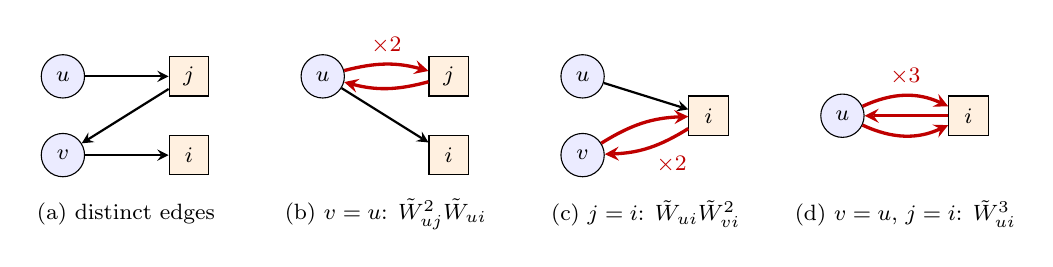
\begin{tikzpicture}[x=1cm,y=1cm,font=\footnotesize,
  un/.style={circle,draw,minimum size=5.5mm,inner sep=0pt,fill=blue!8},
  it/.style={rectangle,draw,minimum size=5mm,inner sep=0pt,fill=orange!12},
  w/.style={->,thick,>=stealth},
  rep/.style={->,very thick,>=stealth,red!75!black}]
\begin{scope}[xshift=0cm]
 \node[un] (u) at (0,1) {$u$}; \node[un] (v) at (0,0) {$v$};
 \node[it] (j) at (1.6,1) {$j$}; \node[it] (i) at (1.6,0) {$i$};
 \draw[w] (u) -- (j); \draw[w] (j) -- (v); \draw[w] (v) -- (i);
 \node at (0.8,-0.75) {(a) distinct edges};
\end{scope}
\begin{scope}[xshift=3.3cm]
 \node[un] (u) at (0,1) {$u$};
 \node[it] (j) at (1.6,1) {$j$}; \node[it] (i) at (1.6,0) {$i$};
 \draw[rep] (u) to[bend left=15] node[above]{$\times2$} (j); \draw[rep] (j) to[bend left=15] (u); \draw[w] (u) -- (i);
 \node at (0.8,-0.75) {(b) $v=u$: $\tW_{uj}^2\tW_{ui}$};
\end{scope}
\begin{scope}[xshift=6.6cm]
 \node[un] (u) at (0,1) {$u$}; \node[un] (v) at (0,0) {$v$};
 \node[it] (i) at (1.6,0.5) {$i$};
 \draw[w] (u) -- (i); \draw[rep] (i) to[bend left=15] node[below right=-1pt]{$\times2$} (v); \draw[rep] (v) to[bend left=15] (i);
 \node at (0.8,-0.75) {(c) $j=i$: $\tW_{ui}\tW_{vi}^2$};
\end{scope}
\begin{scope}[xshift=9.9cm]
 \node[un] (u) at (0,0.5) {$u$};
 \node[it] (i) at (1.6,0.5) {$i$};
 \draw[rep] (u) to[bend left=25] node[above]{$\times3$} (i); \draw[rep] (i) -- (u); \draw[rep] (u) to[bend right=25] (i);
 \node at (0.8,-0.75) {(d) $v=u$, $j=i$: $\tW_{ui}^3$};
\end{scope}
\end{tikzpicture}
\caption{The four kinds of three-hop walks from user $u$ to item $i$. Only walks
of type (a) consist of distinct edges. In (b)--(d) an edge estimate is
multiplied with itself (red), and its power has the wrong mean. DRUP replaces
each repeated factor $\tW_e^k$ by $C_e^kW_e$.}\label{fig:walks}
\end{figure}

\paragraph{Idempotent walk correction}
Let $\Delta=\tW\odot\tW-C\odot C\odot W$, with row sums $r$ and column sums
$\kappa$. The corrected three-hop operator subtracts the excess of each walk
type:
\begin{equation}\label{eq:drup}
\hat T=\tW\tW^\top\tW-\tW\odot(r\mathbf 1^\top-\Delta)-\tW\odot(\mathbf 1\kappa^\top-\Delta)
-(\tW^{\odot3}-C^{\odot3}\odot W).
\end{equation}
The second term removes the excess of type (b) walks, the third removes that of
type (c), and the last removes that of type (d). The subtracted $\Delta$ inside
the first two terms avoids counting type (d) twice. The DRUP score is
$s=a\,\tW+b\,\hat T$.
In the experiments $a=1/c_1$ and $b=\beta/c_3$. Here $c_1$ and $c_3$ are the
mean absolute values of the one- and three-hop terms over all scored users, and
$\beta$ is selected on validation data. The constants are global, so every
user's scores are the same linear combination of the two terms. Within-user
rankings depend on the constants only through $b/a$, so a data-dependent
$c_3/c_1$ acts as a data-dependent rescaling of the grid of $\beta$.
However, $c_1$ and $c_3$ are computed from the log, so
$\E[\hat T/c_3]\neq T^*/c_3$ in general, and the score-level statements below
hold for fixed $a,b$. Constants computed from the imputed graph $C\odot\hat Y$
satisfy Assumption~\ref{as:fixed} whenever $\hat Y$ does. Section~\ref{sec:mc}
compares both choices.

\paragraph{Sample-split variant}
A log rarely comes with an independent log for its nuisances. A sample split
provides one, at a cost. Draw a random set $A$ of pairs, each pair with
probability $q$. Fit $\hat Y$ (and $\hat p$, where it is estimated) on the
pairs in $A$ only. Replace
the edge estimates of the pairs in $A$ by $\hat Y$, take the degrees from
$\hat Y$, and compute $c_1$ and $c_3$ on the imputed graph $C\odot\hat Y$.
Conditionally on $A$ and on the exposures in $A$, the remaining edge estimates
are independent of every nuisance. Assumption~\ref{as:fixed} then holds and the
results below apply, with $\xi_e=\hat Y_e-Y_e$ on the pairs in $A$. The price
is a first-order imputation bias on a fraction $q$ of the pairs, and fewer
exposures for the edge estimates. We call this variant DRUP-split and use
$q=0.2$. The guarantee holds for every fixed configuration. It does not cover
the selection of hyper-parameters on validation data, which every method in our
comparison does and which is outside the guarantee of any estimator.

\paragraph{Public-operator form}
Define the diagonal-corrected item Gram matrix
$G=\tW^\top\tW-\diag(\tW^\top\tW)+\diag(\mathbf 1^\top(C\odot C\odot W))$. Then
\begin{equation}\label{eq:local}
\hat T_{u\cdot}=\tilde w_uG-\tilde w_u\odot(r_u\mathbf 1^\top-2\zeta_u)-(\tilde w_u^{\odot3}-c_u^{\odot3}\odot w_u),
\end{equation}
where $\zeta_u=\tilde w_u^{\odot2}-c_u^{\odot2}\odot w_u$ and lower-case rows
belong to user $u$. Equation~\eqref{eq:local} matches~\eqref{eq:drup} to machine
precision. $G$ is the only object shared across users
(Algorithm~\ref{alg:drup}). Its off-diagonal entries are products of distinct
edges; its diagonal is corrected from $\sum_u\tW_{ui}^2$ to
$\sum_uC_{ui}^2W_{ui}$, the analogue of the diagonal correction of a Gram
matrix estimated from masked data~\citep{lounici2014}.

\begin{algorithm}[t]
\caption{DRUP (training-free)}\label{alg:drup}
\begin{algorithmic}[1]
\Require log $(O,O\odot Y)$; hyper-parameters $\tau,\alpha,\lambda,\beta$
\State fit $\hat p$ (logistic exposure model) and $\hat Y$ (IPS-weighted additive ridge, optionally plus an IPS-weighted low-rank ALS residual), cross-fitted over ten folds of pairs
\State $\bar p\gets\max(\hat p,\tau)$; \ $W\gets\hat Y+O\odot(Y-\hat Y)/\bar p$
\State $C\gets d_u^{-\alpha}d_i^{-(1-\alpha)}$ with $d$ from $\hat Y$
\State $G\gets\tW^\top\tW-\diag(\tW^\top\tW)+\diag(\mathbf 1^\top(C\odot C\odot W))$ \Comment{public operator}
\For{each user $u$ (locally)}
\State $\hat T_{u\cdot}\gets$ Eq.~\eqref{eq:local}; \ $s_u\gets a\,\tilde w_u+b\,\hat T_{u\cdot}$; rank unexposed items by $s_u$
\EndFor
\end{algorithmic}
\end{algorithm}

\paragraph{Control-variate family}
More generally, $W^\lambda_e=O_eY_e/\bar p_e+\lambda(\hat Y_e-O_e\hat Y_e/\bar p_e)$
is unbiased for every $\lambda\in[0,1]$ under correct propensities. It
interpolates between IPS ($\lambda=0$) and DR ($\lambda=1$, the only member that
is also robust to propensity errors). It equals the DR estimate with the
shrunk imputation $\lambda\hat Y$. With $\bar p=p$ its variance is
$\frac{1-p}{p}(Y-\lambda\hat Y)^2$. All results below hold for every member, and
$\lambda$ is selected on validation data.

\paragraph{Imputation and cost}
Theorem~\ref{thm:unbiased} holds for any fixed $\hat Y$. We use an additive model
$\mu+b_u+b_i$ fitted by IPS-weighted ridge regression, or that model plus a rank-32
residual fitted by IPS-weighted alternating least squares. At three hops the
correction costs one $n\times n$ Gram product and $O(mn)$ reductions, which is the cost of the
uncorrected operator. The five-hop correction is 29 times slower (Section~\ref{sec:mc}).
The dense $W$ and $G$ need $O(mn+n^2)$ memory. This limits the present implementation to
catalogues of about $10^4$--$10^5$ items.

%======================================================================
\section{Theory}
%======================================================================

Proofs are in Supplementary Section~S1. Let $\varepsilon_e=|Y_e-\hat Y_e|$.

\subsection{Unbiasedness and its limits}

\begin{theorem}[Edge-wise double robustness]\label{thm:unbiased}
Under Assumptions~\ref{as:unconf}--\ref{as:fixed}, let
$\xi_e=(p_e/\bar p_e-1)(Y_e-\hat Y_e)$. Then $\E[\hat T_{ui}]$ equals $T^*_{ui}$
with every distinct edge contributing $Y_e+\xi_e$ once. In particular, if
every edge has a correct propensity or a correct imputation, then
$\E[s]=F^*$.
\end{theorem}

Recommendations rank the \emph{unexposed} candidates of a user, and there
the candidate's own edge estimate is deterministic ($W_{ui}=\hat Y_{ui}$ for DR,
$0$ for IPS). The following corollary states what DRUP estimates on the
candidate set.

\begin{corollary}[Unexposed candidates]\label{cor:cand}
Under the conditions of Theorem~\ref{thm:unbiased} with $\xi\equiv0$,
\begin{gather*}
\E[s_{ui}\mid O_{ui}=0]=F^*_{ui}-(Y_{ui}-\hat Y_{ui})\,g_{ui},\\
g_{ui}=\frac{\partial F^*_{ui}}{\partial Y_{ui}}
=C_{ui}\Big(a+b\big(\textstyle\sum_{v\neq u}C_{vi}^2Y_{vi}+\sum_{j\neq i}C_{uj}^2Y_{uj}+C_{ui}^2\big)\Big)\ge0 .
\end{gather*}
For IPS edges the same holds with $\hat Y_{ui}=0$. The residual is the
imputation error at the candidate itself. If $p_e$ depends on $Y$ only through
$Y_e$, the log carries no information on $Y_{ui}$ when $O_{ui}=0$, so the
residual is not identified and no estimator can remove it.
\end{corollary}

At three hops the walks through $(u,i)$ are exactly those counted in
$g_{ui}$. With IPS edges they vanish on unexposed candidates, so the uncorrected
IPS operator has no repeated-walk bias there. From five hops on, walks repeat
edges that are not incident to the candidate (for example
$u\!-\!j\!-\!v\!-\!j\!-\!v\!-\!i$), and the bias reappears
(Table~\ref{tab:mc}).

\begin{theorem}[Any odd number of hops]\label{thm:khop}
For $K=2r+1$, a walk $U_0\!-\!J_1\!-\!U_1\!-\cdots-\!U_r\!-\!J_{r+1}$ has user
variables $U_0,\dots,U_r$ and item variables $J_1,\dots,J_{r+1}$, with $U_0=u$
and $J_{r+1}=i$. The equality pattern of an assignment is a pair $\pi$ of set
partitions of the user and item variables, and $\pi$ fixes the multiplicity
$k_e$ of every distinct edge. Let $g_\pi(\sigma)$ be the unconstrained
contraction, over the blocks of a coarser pattern $\sigma\ge\pi$, of
$\prod_eC_e^{k_e}W_e$ (corrected) or of $\prod_e\tW_e^{k_e}$ (plug-in), the
product running over the distinct edges of $\pi$. Then
\[
\hat T^{(K)}=\tW(\tW^\top\tW)^r+\sum_{\pi:\,\exists k_e>1}\ \sum_{\sigma\ge\pi}\mu(\pi,\sigma)\big(g^{\mathrm{corr}}_\pi(\sigma)-g^{\mathrm{plug}}_\pi(\sigma)\big),
\]
with $\mu$ the Möbius function of the product of the two partition lattices,
satisfies $\E\hat T^{(K)}=(\tY\tY^\top)^r\tY$ under the conditions of
Theorem~\ref{thm:unbiased} with $\xi\equiv0$.
\end{theorem}
The number of pairs $(\pi,\sigma)$ is 5, 99 and 2{,}790 for $K=3,5,7$, and for
$K=3$ the construction reduces to Eq.~\eqref{eq:drup}. Theorem~\ref{thm:unbiased},
Corollary~\ref{cor:cand} and Theorem~\ref{thm:fair} carry over to any odd $K$.

Assumption~\ref{as:unconf} excludes slates of fixed size, where exposures in a
user's history are negatively dependent (Coat, for instance, collects exactly
24 ratings per user). The next result bounds the resulting bias.

\begin{proposition}[Exposure dependence within users]\label{prop:dep}
Suppose that exposures are independent across users but may be dependent within
a user's row, with $|\mathrm{Cov}(O_e,O_f\mid Y)|\le\rho\,p_ep_f$ for distinct $e,f$ in
the same row. With correct propensities,
\[
\big|\E\hat T_{ui}-T^*_{ui}\big|\ \le\ \rho\sum_{j\neq i}C_{uj}\Big(\sum_{v\neq u}C_{vj}C_{vi}\,\varepsilon_{vj}\varepsilon_{vi}+C_{uj}C_{ui}\,\varepsilon_{uj}\varepsilon_{ui}\Big).
\]
For slates of $k$ items drawn uniformly without replacement, $\rho\le1/k$, and
$\rho\le1$ for any negatively dependent design. For DR edges the bias is of
second order in the imputation error; for IPS edges ($\varepsilon=Y$) it is of
first order.
\end{proposition}

\begin{theorem}[Repeated-walk bias of uncorrected propagation]\label{thm:lower}
Let the propensities be correct and let $(u,i)$ be a candidate with $O_{ui}=0$.
Relative to the conditional target of Corollary~\ref{cor:cand}, the
uncorrected DR operator $\tW\tW^\top\tW$ has conditional bias
\begin{gather*}
C_{ui}\hat Y_{ui}\big(R_u^{(i)}+K_i\big)-C_{ui}^3\hat Y_{ui}(1-\hat Y_{ui}^2),\\
K_i=\sum_{v\neq u}C_{vi}^2V_{vi},\qquad R_u^{(i)}=\sum_{j\neq i}C_{uj}^2V_{uj},
\end{gather*}
where $V_e=\Var(W_e)=\frac{1-p_e}{p_e}\varepsilon_e^2$. Moreover:
(a) $K_i\ge(1/\max_vp_{vi}-1)\sum_{v\neq u}C_{vi}^2\varepsilon_{vi}^2$, which is unbounded
as the item's propensities vanish;
(b) with clipped propensities $\bar p=\max(p,\tau)$, $\tau\le1/2$, the excess
$C_e^2(\E[W_e^2]-\E[W_e])$ of a doubly traversed edge is at most
$C_e^2(1/\tau-1)\varepsilon_e^2$, with equality at $p_e=\tau$; the worst-case
repeated-walk bias is therefore $\Theta(1/\tau)$;
(c) for IPS edges the conditional bias vanishes at three hops.
DRUP has zero bias relative to the same target.
\end{theorem}
The within-user ranking is affected through $C_{ui}\hat Y_{ui}K_i$, which
up-weights items whose other raters were rarely exposed. The term $R_u^{(i)}$ depends on
$i$ only through one term.

\paragraph{Variance and clipping} The variance of an edge estimate scales with the
imputation error $\varepsilon^2$, not with $Y^2$ as for IPS. The clip $\tau$ trades
variance against a clipping bias, which vanishes when $\hat Y$ is accurate. The bounds
(Theorem~S1 in Supplementary Section~S1) are worst-case and loose by a factor of 70 to
8{,}000 in simulation.

\begin{definition}[Exposure elasticity]\label{def:elast}
For an intervention $do(p_{\cdot i}\leftarrow\pi p_{\cdot i})$ on item $i$'s
exposure mechanism, after which the estimator uses the post-intervention
propensities ($\hat p_{\cdot i}\leftarrow\pi\hat p_{\cdot i}$) and otherwise the same
nuisances, $\eta_i=\partial\log\E[s_{ui}]/\partial\log\pi$.
\end{definition}

\begin{theorem}[Exposure invariance]\label{thm:fair}
Under Assumptions~\ref{as:unconf}--\ref{as:fixed} and $\pi p\ge\tau$, DRUP has
$\eta_i=0$, also conditionally on $O_{ui}=0$: the expected score of every
candidate is unchanged when item $i$'s exposure mechanism is scaled.
Logged-graph propagation with fixed weights $C$ has $\eta_i\ge1$ (popularity
amplification); normalising by logged degrees partly offsets it.
Uncorrected DR propagation has $\eta_i<0$ whenever $\hat Y_{ui}K_i>0$
(over-correction).
\end{theorem}

Exposure invariance is a statement about expected scores. It is not a
distributive fairness criterion. It is also conditional: when many propensities
lie below the clip, $\pi p\ge\tau$ fails and invariance is lost
(Section~\ref{sec:fair}).

\subsection{Structural properties}\label{sec:structsum}

Given its nuisances, $s$ is a fixed linear function of the edge estimates.
Section~S3 of the Supplementary Material states and proves the
consequences. They hold for every linear propagation operator, corrected or
not: exact attributions and minimal counterfactual explanations with frozen
nuisances (Proposition~S2, Theorem~S3), conservative
certificates against injected profiles (Theorem~S4), joint
differential privacy when the population-level nuisances, the
hyper-parameters and the score constants are public (Theorem~S5),
and an exposure-capped allocation solved exactly by min-cost flow
(Theorem~S6). Because they are not specific to DRUP, we report
their empirical behaviour in the Supplementary Material
(Section~S4) and use only the allocation in the main text, as a
decision that compares scores across users (Section~\ref{sec:semisynth}).

%======================================================================
\section{Experimental design}\label{sec:setup}
%======================================================================

\subsection{Datasets}\label{sec:data}

Table~\ref{tab:data} describes the four benchmarks. Each pairs a biased
training log with an unbiased test set, which is what identifies the effect of a
debiasing method: a random sample of ratings (Coat, Yahoo!\,R3), random
impressions (KuaiRand) or a fully observed matrix (KuaiRec). All four are public.

\begin{table}[t]\centering\scriptsize
\caption{Datasets. ``Log'': the biased training data, with its density.
``Test'': the unbiased data. ``Candidates'': unbiased test items per user that are
ranked (items never logged for that user). ``Evaluated users'': users with at
least one positive candidate.}\label{tab:data}
\begin{adjustbox}{max width=\textwidth}
\begin{tabular}{lcccccc}
\toprule
Dataset & Users / items & Log (density) & $O$ means & Test & Candidates & Evaluated users\\
\midrule
Coat & 290 / 300 & 6{,}960 (8.0\%) & Self-rated & 16 random ratings per user & 14.7 & 225\\
Yahoo!\,R3 & 15{,}400 / 1{,}000 & 311{,}704 (2.0\%) & Self-rated & 10 random songs, 5{,}400 users & 10 & 2{,}315\\
KuaiRand & 10{,}000 / 7{,}583 & 511{,}863 (0.68\%) & Feed impression & random impressions & 43.6 & 8{,}347\\
KuaiRec & 7{,}176 / 10{,}728 & 10.3M (13.4\%) & Impression & fully observed 1{,}411 $\times$ 3{,}327 & 3{,}314 & 1{,}411\\
\bottomrule
\end{tabular}

\end{adjustbox}
\end{table}

\emph{Coat}~\citep{schnabel2016} has 290 users, 300 items and 6{,}960
self-selected ratings (24 per user, 8.0\% dense). The test data are 16 ratings per
user on uniformly random items; we rank the items the user did not rate (14.7
candidates on average), and 225 users have a positive candidate. The dataset
ships propensities, which we use.
\emph{Yahoo!\,R3}~\citep{marlin2009collaborative} has 311{,}704 self-selected
ratings of 15{,}400 users on 1{,}000 songs (2.0\% dense) and 54{,}000 ratings of
ten random songs for 5{,}400 of the users, in the version distributed
with~\citep{chen2021autodebias}. A random 5\% of the test users is held out and
used only to fit an outcome-dependent propensity model~\citep{schnabel2016}; in a
preliminary comparison on validation data it did not improve the propagation
operators, so all reported results use a logistic exposure model. The remaining 5{,}130 users have ten
candidates each, and 2{,}315 of them a positive.
\emph{KuaiRand-Pure}~\citep{gao2022kuairand} is the only dataset that records
platform exposure rather than self-selection: $O$ is an impression of the
standard feed and $Y$ a click. We keep a random 10{,}000 of the users who also
received randomly exposed videos, and all 7{,}583 videos; the log has 511{,}863
impressions (0.68\% dense, click rate 47\%). The random impressions of the same
period, restricted to videos the user was not shown in the standard log, are the
test set (43.6 candidates per user, 17.5\% clicked; 8{,}347 users have a
positive). \emph{KuaiRec}~\citep{gao2022kuairec} provides the big matrix (7{,}176
users, 10{,}728 items, 10.3M views, 13.4\% dense) as the log and a fully observed
small matrix (1{,}411 users, 3{,}327 items) as the test set; we rank the 3{,}314
small-matrix items per user that the user never viewed in the log (154 positive
on average).

Positives are ratings $\ge4$ (Coat, Yahoo!\,R3), a watch ratio $\ge2$ (KuaiRec)
and a click (KuaiRand). A random ranking reaches nDCG@5 of 0.306 on Coat and
0.352 on Yahoo!\,R3, nDCG@10 of 0.33 on KuaiRand and nDCG@20 of 0.046 on
KuaiRec, so the candidate sets of Coat and Yahoo!\,R3 compress metric differences.
On Coat and Yahoo!\,R3 ``exposure'' means that the user chose to rate the item,
and exposure invariance is invariance to that choice, not to a platform's
allocation.

\subsection{Baselines}\label{sec:baselines}

We compare DRUP with up to 26 baselines (counting the non-personalised methods and, among the debiased-graph operators,
IPS adjacency with and without the walk correction and EASE, GF-CF and BSPM on the DR graph, but not DR adjacency,
DRUP or their variants), all run by us on the same datasets,
splits and validation data; no number is taken from the literature.
\emph{Non-personalised}: popularity and the imputation $\hat Y$ alone.
\emph{Trained, pointwise loss}: MF, IPS-MF~\citep{schnabel2016}, DR-MF,
DR-JL~\citep{wang2019drjl}, MRDR~\citep{guo2021mrdr}, iALS~\citep{hu2008ials},
LightGCN and DR-LightGCN. \emph{Trained, pairwise or contrastive loss}: MF, PDA~\citep{zhang2021pda},
MACR~\citep{wei2021macr}, LightGCN~\citep{he2020lightgcn},
r-AdjNorm~\citep{zhao2022radjnorm}, NAVIP~\citep{kim2022navip} and
SimGCL~\citep{yu2022simgcl}. \emph{Training-free, logged graph}: linear
LightGCN (with the searched normalisation exponent it is a linear r-AdjNorm),
EASE~\citep{steck2019ease}, GF-CF~\citep{shen2021gfcf} and
BSPM~\citep{choi2023bspm}. \emph{Training-free, debiased graph}: IPS adjacency
(NAVIP-style), IPS with the walk correction, EASE, GF-CF and BSPM on the DR graph,
uncorrected DR adjacency and the five-hop versions. DRUP-split
(Section~\ref{sec:drup}) is run over five draws of the split-off pairs. Grids and
training details are in Supplementary Section~S2.

\paragraph{How recent are the baselines?} The most recent are BSPM (2023),
SimGCL, r-AdjNorm and NAVIP (2022) and MRDR (2021), which are among the
strongest published graph, contrastive and debiased models for implicit
feedback and which are open for re-implementation on the biased-log-plus-random-test
protocol; DR-JL (2019) is included because the DR baseline is the direct
ancestor of our edge estimate. We did not run StableDR, DICE, CausE or AutoDebias
because they either need the uniform data for training (CausE, AutoDebias), which
our protocol keeps for selection and testing, or are covered by the
corresponding DR and popularity baselines (StableDR, DICE).

\paragraph{Large language models} We did not compare with LLM-based
recommenders. Our pipeline uses only interaction data: the four benchmarks come
with no item or user text that we use, and the question studied here is how to
estimate a propagation operator under exposure bias, for which the relevant
comparators are graph operators. A comparison with LLM-based recommenders would
need a dataset that has item text and a random-exposure test set, which none of our
benchmarks provides together, and it would test a different hypothesis, that text
helps. We list this as a limitation (Section~\ref{sec:disc}).

\subsection{Protocol}\label{sec:protocol}

The unbiased data are split into validation (30\% of each user's candidates on
Coat, 30\% of the test users otherwise) and test parts over 10 (Coat) or 5 random
splits. Every method selects its configuration on the validation part of each
split, and trained models also select their epoch there: each split stops on its
own validation score and never sees the validation or test users of another split.
Nuisances are cross-fitted over ten folds of pairs, except for the sample-split
variants, whose imputation (and propensity model, where it is estimated) is fitted
on a random 20\% of the pairs; only the latter satisfy the assumptions of the
theory (Remark~\ref{rem:xfit}). We report nDCG@5 on Coat and Yahoo!\,R3, nDCG@10
on KuaiRand and nDCG@20 on KuaiRec (AUC and Recall are in the Supplementary
Material) as the mean and standard deviation over splits. Differences are tested
at the level of users, with a Holm correction over all comparisons of a dataset;
paired tests over overlapping splits are anti-conservative~\citep{nadeau2003}, so
we add the corrected resampled test over splits and equivalence tests for the
key comparisons (Supplementary Table~S19). The tests treat the training log,
the fitted nuisances and the trained models as fixed. Because progress claims in
top-$N$ recommendation have repeatedly failed against tuned simple
baselines~\citep{dacrema2019progress,rendle2019baselines,anelli2023myth}, every
method is tuned on the same validation data, and the number of configurations
each searched is reported (Supplementary Section~S2).


%======================================================================
\section{Results}\label{sec:results}
%======================================================================

\subsection{Simulation: does the correction work, and under which conditions?}\label{sec:mc}

This section addresses RQ1 and RQ2. Table~\ref{tab:mc} uses a synthetic MNAR model
with known propensities: 30 users, 40 items, low-rank preferences, and exposures
driven by user activity, item popularity and the outcome itself (median
propensity 0.06). We draw 20{,}000 exposure matrices for three hops and 4{,}000 for
five hops.

\begin{table}[t]\centering\small
\caption{Monte-Carlo check of Theorems~\ref{thm:unbiased}, \ref{thm:khop}, \ref{thm:lower}
and~\ref{thm:fair} and Corollary~\ref{cor:cand}. Relative $|$bias$|$ is the mean absolute
bias divided by the mean target, over all entries and conditionally on unexposed
candidates (against the conditional target of Corollary~\ref{cor:cand}). Kendall
$\tau$ is the mean within-user rank agreement of one realisation with the
full-exposure target on unexposed candidates. $\eta$ is the exposure elasticity
(separate model, 3{,}000 replications).}\label{tab:mc}
\begin{adjustbox}{max width=\textwidth}
\begin{tabular}{lcccc}
\toprule
Estimator & rel.\,|bias| & frac.\ $|z|>3$ & rel.\,RMSE & exposure elasticity $\eta$\\
\midrule
Obs & 0.992 & 1.0000 & 1.02 & +1.777\\
IPS & 2.403 & 0.4042 & 21.01 & +0.007\\
IPS+WC & 0.028 & 0.0025 & 4.93 & +0.007\\
DR & 1.903 & 0.6292 & 20.94 & -0.187\\
DRUP & 0.020 & 0.0008 & 3.97 & +0.005\\
\bottomrule
\end{tabular}

\end{adjustbox}
\end{table}

\paragraph{The bias is large and the correction removes it (RQ1)} Over all entries, the
uncorrected IPS and DR operators are biased by 2.3 and 1.8 times the mean target
at three hops and by 15 and 8 times at five hops. With the correction the residual
bias (0.02--0.06) is at the Monte-Carlo error. On the unexposed candidates that are
actually ranked, Corollary~\ref{cor:cand} predicts that IPS is unbiased at three
hops but not at five, and the uncorrected DR operator is biased at both depths;
the simulation agrees (IPS 0.029 at three hops and 4.7 at five; DR 1.1 and 5.1).
The exposure elasticity is $+1.78$ for the logged graph, $-0.19$ for DR adjacency
and $+0.005$ for DRUP. The $K$-hop engine matches the closed-form three-hop
operator to $9\times10^{-16}$ and brute-force enumeration of all five-hop walks to
$10^{-14}$ (absolute error on random $5\times6$ matrices; Supplementary code \texttt{check\_khop.py}). On a dense matrix of KuaiRec's size (7{,}176 users, 10{,}728 items, 1{,}411
scored users, four CPU cores) the corrected three-hop operator takes 1.9\,s against
1.4\,s for the plug-in one, and the corrected five-hop operator 85\,s against
2.9\,s: the correction is exact but not free beyond three hops.

\paragraph{Unbiasedness does not buy ranking accuracy} The rank agreement of one
realisation with the target is higher for the uncorrected DR operator (Kendall
$\tau=0.20$) than for DRUP (0.12). On unexposed candidates the bias is
$C_{ui}\hat Y_{ui}(R_u^{(i)}+K_i)$ (Theorem~\ref{thm:lower}), which adds a
positive multiple of the imputation to the score, and here the imputation is
informative. For IPS edges, whose bias does not involve the imputation, the
correction leaves the rank agreement unchanged.

\begin{table}[t]\centering\small
\caption{Monte-Carlo check of the nuisance protocol (Remark~\ref{rem:xfit}): relative
$|$bias$|$ of the three-hop term against the full-exposure target with the same
weights $C$, over all entries, with true propensities. Nuisances are fitted on
an independent log (Assumption~\ref{as:fixed}), cross-fitted over ten folds of
pairs of the same log (the protocol of the main experiments), or fitted on a
random 50\% or 20\% of the pairs of the same log (sample split). Model: users
$\times$ items and mean exposures per user; the last model has three times larger
propensities. The last two columns give the bias of the full score
$s=s_1/c_1+s_3/c_3$ with constants computed from the scores or from the imputed
graph (2{,}000--3{,}000 replications).}\label{tab:protocol}
\begin{adjustbox}{max width=\textwidth}
\begin{tabular}{llcccccc}
\toprule
 & & \multicolumn{2}{c}{IPS edges} & \multicolumn{4}{c}{DR edges}\\
Model & Nuisances & uncorr. & DRUP & uncorr. & DRUP & $s$, data $c$ & $s$, $\hat Y$ $c$\\
\midrule
40$\times$60, 11 & independent log & 2.15 & 0.10 & 1.90 & 0.09 & 0.35 & 0.11\\
 & cross-fitted (protocol) & 0.39 & 0.64 & 0.61 & 0.80 & 0.62 & 0.88\\
 & cross-fitted, $W$-degrees & 3.12 & 0.81 & 4.11 & 0.73 & 0.49 & 2.69\\
 & sample split, 50\% & 0.60 & 0.42 & 0.55 & 0.42 & 0.35 & 0.63\\
 & sample split, 20\% & 1.09 & 0.17 & 0.90 & 0.17 & 0.29 & 0.24\\
\midrule
60$\times$120, 23 & independent log & 0.98 & 0.07 & 0.82 & 0.06 & 0.30 & 0.07\\
 & cross-fitted (protocol) & 0.31 & 0.52 & 0.42 & 0.61 & 0.42 & 0.58\\
 & cross-fitted, $W$-degrees & 1.51 & 0.69 & 1.80 & 0.58 & 0.40 & 1.09\\
 & sample split, 50\% & 0.32 & 0.39 & 0.31 & 0.39 & 0.35 & 0.52\\
 & sample split, 20\% & 0.54 & 0.18 & 0.47 & 0.18 & 0.26 & 0.26\\
\midrule
60$\times$120, 60 & independent log & 0.15 & 0.01 & 0.09 & 0.01 & 0.18 & 0.02\\
 & cross-fitted (protocol) & 0.11 & 0.17 & 0.12 & 0.18 & 0.20 & 0.12\\
 & cross-fitted, $W$-degrees & 0.17 & 0.18 & 0.11 & 0.12 & 0.18 & 0.08\\
 & sample split, 50\% & 0.09 & 0.13 & 0.10 & 0.13 & 0.35 & 0.33\\
 & sample split, 20\% & 0.09 & 0.07 & 0.07 & 0.07 & 0.23 & 0.14\\
\bottomrule
\end{tabular}

\end{adjustbox}
\end{table}

\paragraph{The guarantees do not survive data-dependent weights (RQ2)}
Table~\ref{tab:protocol} measures the guarantees under the ways nuisances are
fitted in practice. With nuisances from an independent log the corrected operator is
at the Monte-Carlo error (0.01--0.10), while the uncorrected operators are biased by
0.09--2.2 times the mean target. Under the cross-fitted protocol of our main
experiments the advantage disappears: the corrected operator is biased by
0.17--0.80 and the uncorrected one by 0.11--0.61, because the degree weights
depend on the exposures of the walk edges. A control that fixes the degree weights
a priori (Table~S18 in the Supplementary Material) isolates the
cause: with fixed weights, cross-fitting alone preserves the correction (IPS with the
correction 0.05 against 1.10 uncorrected; DRUP 0.05 against 0.89), whereas degrees
from the cross-fitted $\hat Y$ or from the edge estimates destroy it (0.64--0.80 and
0.74--0.82). Fitting the nuisances in sample breaks the correction even with fixed
weights for DR edges (0.23). The sample split restores the guarantee: relative to
the target of Theorem~\ref{thm:unbiased}, the bias of DRUP-split is 0.004--0.066, and
relative to the full-exposure target 0.07--0.18 at $q=0.2$, against 0.07--1.09 for
the uncorrected operator under the same split. The data-dependent constants matter
too: with independent nuisances and DR edges, the full score is biased by 0.18--0.35
when $c_1,c_3$ are computed from the scores and by 0.02--0.11 when they come from the
imputed graph. Stress tests (fixed-size slates, misspecified propensities, bounds on
the variance) are in the Supplementary Material.

\subsection{Score values on a semi-synthetic KuaiRec log (RQ3, part 1)}\label{sec:semisynth}

\begin{table}[t]\centering\small
\caption{Semi-synthetic KuaiRec (30 draws of the log). RMSE $T$: root mean
squared error of the three-hop term over all pairs, relative to the root
mean square of the target (only for fixed $C$, where estimator and target use
the same weights). Utility error: relative error (mean $\pm$ standard error over
draws) of the estimated full-exposure utility $\sum_x s$ of a fixed random and a
fixed popular allocation of 20 unexposed items per user. Regret: loss of
full-exposure utility of the exposure-capped allocation computed from the
estimated scores, relative to the one computed from $F^*$. nDCG@20 against $Y$
on unexposed items. True propensities; estimated ones and a sparser log are
in the Supplementary Material.}\label{tab:semisynth}
\begin{adjustbox}{max width=\textwidth}
\begin{tabular}{llllccccc}
\toprule
 & & & & & \multicolumn{2}{c}{utility error (\%)} & & \\
$p$ & Nuisances & $C$ & Estimator & RMSE $T$ & random & popular & regret & nDCG@20\\
\midrule
true & independent log & fixed & IPS & 22.8 & +17.8$\pm$4.0 & +10.3$\pm$0.4 & 0.795 & 0.097\\
 &  &  & IPS+WC & 2.9 & +0.4$\pm$1.2 & +0.4$\pm$0.3 & 0.795 & 0.097\\
 &  &  & DR & 28.2 & +23.0$\pm$4.9 & +17.8$\pm$0.5 & 0.791 & 0.097\\
 &  &  & DRUP & 6.3 & -1.8$\pm$1.4 & -0.0$\pm$0.4 & 0.795 & 0.107\\
\midrule
true & independent log & $\hat Y$ & IPS & -- & -44.0$\pm$1.0 & -41.3$\pm$0.2 & -- & 0.120\\
 &  &  & IPS+WC & -- & -48.4$\pm$0.8 & -44.4$\pm$0.2 & -- & 0.120\\
 &  &  & DR & -- & -44.0$\pm$1.0 & -40.4$\pm$0.2 & -- & 0.377\\
 &  &  & DRUP & -- & -49.3$\pm$0.8 & -44.6$\pm$0.2 & -- & 0.370\\
\midrule
true & cross-fitted & fixed & IPS & 22.8 & +17.8$\pm$4.0 & +10.3$\pm$0.4 & 0.795 & 0.097\\
 &  &  & IPS+WC & 2.9 & +0.4$\pm$1.2 & +0.4$\pm$0.3 & 0.795 & 0.097\\
 &  &  & DR & 35.3 & +28.6$\pm$4.7 & +18.9$\pm$0.5 & 0.821 & 0.051\\
 &  &  & DRUP & 8.5 & -0.1$\pm$1.6 & +0.8$\pm$0.4 & 0.819 & 0.068\\
\midrule
true & cross-fitted & $\hat Y$ & IPS & -- & -54.0$\pm$0.7 & -46.5$\pm$0.1 & -- & 0.191\\
 &  &  & IPS+WC & -- & -56.3$\pm$0.6 & -48.5$\pm$0.1 & -- & 0.191\\
 &  &  & DR & -- & -53.7$\pm$0.9 & -45.4$\pm$0.1 & -- & 0.320\\
 &  &  & DRUP & -- & -57.4$\pm$0.8 & -48.8$\pm$0.1 & -- & 0.322\\
\midrule
true & sample split & fixed & IPS & 20.6 & +53.2$\pm$3.9 & +55.9$\pm$0.6 & 0.822 & 0.093\\
 &  &  & IPS+WC & 2.5 & +37.9$\pm$1.2 & +47.2$\pm$0.6 & 0.821 & 0.091\\
 &  &  & DR & 103.6 & +63.3$\pm$5.0 & +63.7$\pm$0.8 & 0.840 & 0.030\\
 &  &  & DRUP & 8.8 & +37.9$\pm$1.5 & +47.0$\pm$0.6 & 0.837 & 0.048\\
\midrule
true & sample split & $\hat Y$ & IPS & -- & +0.8$\pm$1.9 & -10.4$\pm$0.6 & -- & 0.154\\
 &  &  & IPS+WC & -- & -10.7$\pm$1.3 & -17.1$\pm$0.5 & -- & 0.150\\
 &  &  & DR & -- & +0.9$\pm$1.8 & -10.3$\pm$0.6 & -- & 0.274\\
 &  &  & DRUP & -- & -10.8$\pm$1.2 & -17.2$\pm$0.5 & -- & 0.272\\
\midrule
\multicolumn{9}{l}{Five hops (independent log, true $p$, fixed $C$): relative $|$bias$|$ of $T_5$, DR 3.46, DRUP 0.32.}\\
\bottomrule
\end{tabular}

\end{adjustbox}
\end{table}

On real benchmarks the full-exposure target $F^*$ is unknown, so they cannot show
whether score values are right. We therefore use KuaiRec's fully observed small matrix
(1{,}411 users, 3{,}327 items, 4.6\% positives) as the potential outcomes $Y$ and
draw exposure logs from a known MNAR mechanism fitted to the big matrix,
$\operatorname{logit}p_{ui}=c+z_u+1.5z_i+Y_{ui}$, with $z$ the standardised logit
exposure rates of the user and the item in the big log and $c$ set for a
density of 13\% as in the big matrix (median propensity 0.064, all
propensities at least $\tau=0.02$). The target uses weights $C$ fixed a priori
(degrees of $Y$, $\alpha=0.5$) and $a,b$ fixed from the target. Each estimator
uses either the same fixed $C$ or degrees from its imputation (as in our
real-data configurations), a rank-16 IPS-weighted imputation, and nuisances
from an independent log, cross-fitted on the same log, or from the 20\% sample
split. Table~\ref{tab:semisynth} reports score errors and three uses of the
scores.

\paragraph{Score values} With true propensities and fixed weights, the
correction lowers the relative RMSE of the three-hop term by a factor of 4 to
12 (IPS 22.8 to 2.9, DR 28.2 to 6.3 with an independent log; DR 35.3 to 8.5
cross-fitted): the repeated factors of rarely exposed edges dominate the error
as well as the bias. With 30 draws the remaining three-hop bias of the
corrected operators is within Monte-Carlo error; at five hops the relative
bias drops from 3.46 (DR) to 0.32 (DRUP). The difference shows in a quantity
that uses score values: the sum of the scores of a fixed allocation estimates its
full-exposure utility, and the uncorrected operators overestimate it by 18--29\% (random allocation) and 10--19\% (popular items),
whereas IPS with the correction and DRUP are within 2\% of the truth. This
holds with an independent log and, because $C$ is fixed, also with
cross-fitted nuisances (DRUP $-0.1\pm1.6\%$ against DR $+28.6\pm4.7\%$). The
sample split removes the dependence but imputes a fifth of the pairs, and its
imputation bias shifts the corrected estimates up by 38--47\% (uncorrected:
53--64\%).

\paragraph{What does not change} Two uses of the scores are unaffected. The
exposure-capped allocation, which compares scores across users, loses 79--84\%
of the achievable full-exposure utility under every estimator: per-pair noise,
not the repeated-walk bias, decides which pairs are allocated. Rankings do not
improve either: with imputation-based weights, DR adjacency and DRUP reach
nDCG@20 of 0.377 and 0.370. With weights taken from the imputation, finally,
every operator estimates a different, imputation-indexed quantity; with an
independent log or cross-fitted nuisances it is off by 40--57\% in utility
against the fixed-weight target, corrected or not, so score values need
weights fixed a priori. With estimated propensities all estimators
overstate utility by 100--540\%, and the propensity model, not the walk
correction, dominates the error (Table~S14).

\paragraph{A sparser log} At a density of 3\% (median propensity 0.008, 58\% of
the propensities below the clip $\tau=0.01$) the conditions of the theorems
fail, and clipping dominates (Table~S15). The correction
still lowers the three-hop RMSE by a factor of 7 to 32, but every utility
estimate is biased: IPS with the correction by $-28\%$, DR adjacency by $+331\%$
and DRUP by $+164\%$ with an independent log, in line with the clipping bias of
Theorem~S1(c).


\subsection{Accuracy on unbiased test data (RQ3, part 2)}\label{sec:acc}

\begin{table}[t]\centering\small
\caption{Accuracy on unbiased test data (mean$\pm$std over splits; for the
sample-split rows, mean$\pm$std over five draws of the split-off pairs). Best in
bold, second underlined. ``--'': not run (five hops only where the three-hop DR
operators are competitive). Every method is tuned per split on the same
validation data; Table~S1 lists the number of configurations.
Only the sample-split variants satisfy Assumption~\ref{as:fixed}.}\label{tab:acc}
\begin{adjustbox}{max width=\textwidth}
\begin{tabular}{llcccc}
\toprule
 & Method & Coat nDCG@5 & Yahoo!\,R3 nDCG@5 & KuaiRand nDCG@10 & KuaiRec nDCG@20\\
\midrule
\multicolumn{6}{l}{\emph{Non-personalised}}\\
 & Popularity & 0.5367$\pm$0.0095 & 0.5331$\pm$0.0059 & -- & 0.5766$\pm$0.0023\\
 & Imputation only & 0.5532$\pm$0.0097 & 0.5162$\pm$0.0044 & -- & 0.6194$\pm$0.0018\\
\multicolumn{6}{l}{\emph{Trained, pointwise loss}}\\
 & MF & 0.4780$\pm$0.0168 & 0.5076$\pm$0.0060 & -- & 0.6227$\pm$0.0029\\
 & IPS-MF & 0.4713$\pm$0.0160 & 0.5098$\pm$0.0048 & -- & 0.6258$\pm$0.0025\\
 & DR-MF & 0.5237$\pm$0.0111 & 0.5116$\pm$0.0020 & -- & 0.6191$\pm$0.0020\\
 & DR-JL & 0.4811$\pm$0.0164 & -- & -- & --\\
 & MRDR & 0.4869$\pm$0.0187 & -- & -- & --\\
 & iALS & \textbf{0.5812$\pm$0.0101} & -- & -- & --\\
 & LightGCN & 0.5389$\pm$0.0107 & 0.5935$\pm$0.0059 & -- & 0.6277$\pm$0.0027\\
 & DR-LightGCN & 0.5724$\pm$0.0205 & 0.5440$\pm$0.0029 & -- & 0.6246$\pm$0.0016\\
\multicolumn{6}{l}{\emph{Trained, pairwise or sampled loss}}\\
 & MF (BPR) & 0.5174$\pm$0.0206 & 0.6460$\pm$0.0041 & -- & 0.5913$\pm$0.0028\\
 & PDA & 0.5181$\pm$0.0138 & 0.6516$\pm$0.0052 & -- & 0.5822$\pm$0.0020\\
 & MACR & 0.5418$\pm$0.0134 & -- & -- & --\\
 & LightGCN (BPR) & 0.5683$\pm$0.0132 & 0.6693$\pm$0.0045 & -- & 0.6086$\pm$0.0028\\
 & r-AdjNorm & 0.5722$\pm$0.0134 & \textbf{0.6713$\pm$0.0050} & -- & 0.6086$\pm$0.0031\\
 & NAVIP & 0.5664$\pm$0.0163 & \underline{0.6694$\pm$0.0059} & -- & 0.6183$\pm$0.0024\\
 & SimGCL & 0.5528$\pm$0.0141 & -- & -- & --\\
\multicolumn{6}{l}{\emph{Training-free, logged graph}}\\
 & linear LightGCN / r-AdjNorm & 0.5571$\pm$0.0100 & 0.6585$\pm$0.0058 & -- & 0.6036$\pm$0.0028\\
 & EASE & 0.5401$\pm$0.0138 & 0.6478$\pm$0.0061 & -- & 0.5213$\pm$0.0032\\
 & GF-CF & 0.5513$\pm$0.0123 & 0.6552$\pm$0.0039 & -- & 0.6141$\pm$0.0025\\
 & BSPM & \underline{0.5727$\pm$0.0090} & 0.6507$\pm$0.0047 & -- & --\\
\multicolumn{6}{l}{\emph{Training-free, debiased graph}}\\
 & IPS adjacency (NAVIP-style) & 0.5510$\pm$0.0224 & 0.6567$\pm$0.0063 & -- & 0.6132$\pm$0.0030\\
 & IPS + walk correction & 0.5510$\pm$0.0224 & 0.6567$\pm$0.0063 & -- & 0.6132$\pm$0.0030\\
 & EASE on DR graph & 0.5564$\pm$0.0141 & 0.6072$\pm$0.0033 & -- & 0.6026$\pm$0.0022\\
 & GF-CF on DR graph & 0.5608$\pm$0.0083 & 0.6312$\pm$0.0051 & -- & 0.6371$\pm$0.0021\\
 & BSPM on DR graph & 0.5624$\pm$0.0112 & 0.6262$\pm$0.0071 & -- & --\\
 & DR adjacency & 0.5459$\pm$0.0244 & 0.6567$\pm$0.0063 & -- & \underline{0.6378$\pm$0.0020}\\
 & DRUP & 0.5467$\pm$0.0235 & 0.6567$\pm$0.0063 & -- & 0.6378$\pm$0.0019\\
 & DR adjacency, 5 hops & 0.5524$\pm$0.0245 & -- & -- & \textbf{0.6379$\pm$0.0011}\\
 & DRUP, 5 hops & 0.5451$\pm$0.0204 & -- & -- & 0.6376$\pm$0.0011\\
\multicolumn{6}{l}{\emph{Training-free, sample split (Assumption 2 holds)}}\\
 & DR adjacency, sample split & 0.5604$\pm$0.0132 & 0.5934$\pm$0.0063 & -- & 0.6338$\pm$0.0013\\
 & DRUP-split & 0.5578$\pm$0.0144 & 0.5925$\pm$0.0051 & -- & 0.6337$\pm$0.0013\\
\bottomrule
\end{tabular}

\end{adjustbox}
\end{table}

\begin{table}[t]\centering\small
\caption{User-level paired comparisons: mean difference of the test metric
over users with a 95\% interval, and the $t$-test $p$-value, Holm-adjusted over
all comparisons run for the dataset (DRUP, DR adjacency and DRUP-split, and on Coat and KuaiRec also five-hop DRUP, each
against every other method: 124 on Coat, 87 on Yahoo!\,R3, 75 on KuaiRand, 124 on KuaiRec). Users with a positive
candidate who are in the test part of at least one split (225, 2{,}310, 8{,}321 and
1{,}410); sample-split rows use the first draw. Selected rows; all comparisons
are in the result files.}\label{tab:sig}
\begin{adjustbox}{max width=\textwidth}
\begin{tabular}{lcccccc}
\toprule
DRUP against & \multicolumn{2}{c}{Coat} & \multicolumn{2}{c}{Yahoo!\,R3} & \multicolumn{2}{c}{KuaiRec}\\
 & $\Delta$ [95\% CI] & $p_{\mathrm{Holm}}$ & $\Delta$ [95\% CI] & $p_{\mathrm{Holm}}$ & $\Delta$ [95\% CI] & $p_{\mathrm{Holm}}$\\
\midrule
DR adjacency (effect of the correction) & +0.0020 [-0.003, +0.007] & 1.000 & -- & -- & -- & --\\
DR adjacency, 5 hops (effect of the correction) (5 hops) & -- & -- & -- & -- & -- & --\\
linear LightGCN on the logged graph & -0.0097 [-0.049, +0.029] & 1.000 & -- & -- & -- & --\\
imputation only & -0.0057 [-0.016, +0.004] & 1.000 & -- & -- & -- & --\\
GF-CF & -0.0043 [-0.043, +0.034] & 1.000 & -- & -- & -- & --\\
EASE & +0.0061 [-0.033, +0.045] & 1.000 & -- & -- & -- & --\\
GF-CF on DR graph & -0.0102 [-0.017, -0.004] & 0.058 & -- & -- & -- & --\\
EASE on DR graph & -0.0074 [-0.021, +0.006] & 1.000 & -- & -- & -- & --\\
LightGCN (BPR) & -0.0248 [-0.058, +0.008] & 1.000 & -- & -- & -- & --\\
r-AdjNorm & -0.0294 [-0.063, +0.004] & 1.000 & -- & -- & -- & --\\
NAVIP & -0.0212 [-0.054, +0.012] & 1.000 & -- & -- & -- & --\\
MF (BPR) & +0.0372 [+0.007, +0.067] & 0.287 & -- & -- & -- & --\\
DR-MF & +0.0235 [+0.002, +0.045] & 0.627 & -- & -- & -- & --\\
PDA & +0.0277 [-0.004, +0.060] & 1.000 & -- & -- & -- & --\\
DR-LightGCN & +0.0004 [-0.021, +0.022] & 1.000 & -- & -- & -- & --\\
\bottomrule
\end{tabular}

\end{adjustbox}
\end{table}

Tables~\ref{tab:acc} and~\ref{tab:sig} report accuracy and the user-level tests;
AUC and Recall are in the Supplementary Material and lead to the same conclusions.

\paragraph{The walk correction does not change accuracy} DRUP and the uncorrected
DR adjacency with the same grid are not significantly different (Coat $+0.0014$,
KuaiRec $-0.0001$, $p_{\mathrm{Holm}}=1$). Only KuaiRec and, marginally, Coat can
test equivalence: within $\pm0.005$ nDCG the two operators are equivalent on KuaiRec
($p_{\mathrm{TOST}}<10^{-3}$, also at $\pm0.002$) and marginally so on Coat
($p_{\mathrm{TOST}}=0.034$, but 0.38 at $\pm0.002$; Table~S19). The margin
is a convention, about twice the split-to-split standard deviation of the methods on
KuaiRec (0.002--0.004). On Yahoo!\,R3 and KuaiRand the two operators coincide
exactly, so there is nothing to test: validation selects the IPS end of the
control-variate family ($\lambda=0$) on every split, and IPS edges have no three-hop
repeated-walk bias on unexposed candidates (Corollary~\ref{cor:cand}). At five hops,
where the correction is active for both edge types, the corrected operator is lower
by 0.0003 nDCG@20 on KuaiRec ($p_{\mathrm{Holm}}=0.17$) and by 0.008 nDCG@5 on Coat
($p_{\mathrm{Holm}}=1$); five hops do not add accuracy over three.

\paragraph{The sample split costs accuracy on sparse logs} DRUP-split, the only
variant covered by the guarantees, reaches $0.632\pm0.004$ on KuaiRec over five draws
of the split-off pairs (0.006 below cross-fitted DRUP), $0.544\pm0.011$ on Coat (0.527
to 0.558: which fifth of 24 ratings per user feeds the nuisances matters),
$0.440\pm0.001$ on KuaiRand (0.009 below) and $0.595\pm0.004$ on Yahoo!\,R3 (0.062
below, $p_{\mathrm{Holm}}<10^{-3}$), where a fifth of the few logged exposures goes
to the nuisances and the imputation that replaces them is poor.
DRUP-split and DR adjacency under the same split are not significantly different on any dataset.

\paragraph{Which method is most accurate depends on the dataset}
\emph{KuaiRec.} Training-free propagation over the DR graph reaches nDCG@20 of 0.638,
ahead of every trained model at the user level but by little over the best: DR-JL and
MRDR (0.633; $+0.004$, $p_{\mathrm{Holm}}=0.003$). With the Nadeau--Bengio test over
splits, adjusted over the same family, neither margin is significant
($p_{\mathrm{NB,Holm}}=1.0$ and 0.34), and both are smaller than the seed spread of these
models (0.009 and 0.015). The margin over pointwise LightGCN (0.627; $+0.010$) is
significant under both tests. GF-CF on the DR graph performs as well as DRUP (0.637).
Propagating the imputation alone, with no observed residual, reaches 0.631: two thirds of
the 0.018 that DRUP gains over the imputation (0.619) comes from propagating the
imputation. \emph{KuaiRand.} DRUP, DR adjacency and IPS adjacency coincide (nDCG@10 0.449),
are not significantly different from GF-CF (0.450), BSPM (0.450) or iALS (0.453), and are
significantly behind the BPR graph models: r-AdjNorm 0.459, LightGCN 0.457, NAVIP 0.457
($p_{\mathrm{Holm}}<10^{-3}$). \emph{Yahoo!\,R3.} The imputation alone is below popularity
(0.516 against 0.533), so validation selects IPS edges ($\lambda=0$) with cross-fitted
$W$-degrees, outside Assumption~\ref{as:fixed}; DRUP (0.657) is on par with the logged
graph (0.659) and iALS (0.663) and significantly behind r-AdjNorm (0.674; $-0.019$,
$p_{\mathrm{Holm}}<10^{-3}$), LightGCN and NAVIP. \emph{Coat.} iALS is the most accurate
(0.581), then BSPM, DR-LightGCN and the BPR graph models (0.566--0.573); DRUP reaches 0.547.
After the Holm adjustment over 124 comparisons DRUP is ahead of pointwise MF, IPS-MF,
DR-JL and MRDR only.

\paragraph{Tuning budgets and seed noise} The training-free operators search 384 to
6{,}300 configurations against 6 to 108 for the trained models (Supplementary Table~S1). At the six configurations of DR-JL, the expected KuaiRec score of
DRUP is 0.618 against 0.633 (Supplementary Table~S2); counted in validation
evaluations, which include every epoch of a trained model, DRUP with the 103 evaluations
of DR-JL reaches 0.636. Re-training the split-0 selection of the trained models with other
seeds changes their score by up to 0.013 on Yahoo!\,R3 and 0.075 on Coat (PDA; r-AdjNorm
0.521--0.566), and by 0.009 and 0.015 on KuaiRec for DR-JL and MRDR, so differences on
Coat and the KuaiRec margin over DR-JL and MRDR should be read with this in mind. The loss
matters more than the architecture, in opposite directions: pairwise training is decisive
on Yahoo!\,R3 and KuaiRand (pointwise MF variants stay near 0.51 and 0.37), while on
KuaiRec the pointwise models beat their BPR versions. No single trained baseline is strong
on all datasets.

\subsection{Exposure invariance on real data (RQ4)}\label{sec:fair}

\begin{table}[t]\centering\small
\caption{Real-data intervention $do(p\leftarrow p/2)$: the logged exposures of a
random half of the items are thinned with probability $1/2$ (three to five
draws). Rank shift: change of the treated items' mean within-user rank
relative to control items (0: invariant). $\eta$: elasticity of the mean score
of treated relative to control candidates (1: exposure-proportional, 0:
invariant). Frozen: imputation and degree weights $C$ are kept, the propensities
are updated to the known $p/2$; re-fitted: all nuisances are re-fitted on the thinned
log, with the known propensity change or with propensities re-estimated on it. One configuration
per operator (the one selected most often), all test data.}\label{tab:interv}
\begin{adjustbox}{max width=\textwidth}
\begin{tabular}{llcccccc}
\toprule
 & & \multicolumn{2}{c}{frozen nuisances} & \multicolumn{2}{c}{re-fitted, known $p/2$} & \multicolumn{2}{c}{re-fitted, re-estimated $\hat p$}\\
Data & Operator & rank shift & $\eta$ & rank shift & $\eta$ & rank shift & $\eta$\\
\midrule
Coat & logged graph & -0.0670 & +1.031 & -0.0585 & +0.748 & -- & --\\
 & IPS adjacency & -0.0652 & +0.899 & -0.0651 & +0.900 & -- & --\\
 & DR adjacency & +0.0021 & -0.005 & +0.0001 & -0.019 & -- & --\\
 & DRUP & +0.0036 & -0.008 & +0.0015 & -0.022 & -- & --\\
 & \multicolumn{7}{l}{\footnotesize treated logged pairs below the DRUP clip after $do(p\leftarrow p/2)$: 94\%}\\
\midrule
Yahoo!\,R3 & logged graph & -0.1611 & +1.002 & -0.0943 & +0.508 & -0.0943 & +0.508\\
 & IPS adjacency & -0.1504 & +0.959 & -0.0864 & +0.481 & -0.0873 & +0.485\\
 & DR adjacency & -0.1504 & +0.959 & -0.0864 & +0.481 & -0.0873 & +0.485\\
 & DRUP & -0.1504 & +0.959 & -0.0864 & +0.481 & -0.0873 & +0.485\\
 & \multicolumn{7}{l}{\footnotesize treated logged pairs below the DRUP clip after $do(p\leftarrow p/2)$: 95\%}\\
\midrule
KuaiRand & logged graph & -0.0826 & +0.997 & -0.0679 & +0.711 & -0.0679 & +0.711\\
 & IPS adjacency & -0.0678 & +0.639 & -0.0681 & +0.651 & -0.0680 & +0.653\\
 & DR adjacency & -0.0678 & +0.639 & -0.0681 & +0.651 & -0.0680 & +0.653\\
 & DRUP & -0.0678 & +0.639 & -0.0681 & +0.651 & -0.0680 & +0.653\\
 & \multicolumn{7}{l}{\footnotesize treated logged pairs below the DRUP clip after $do(p\leftarrow p/2)$: 57\%}\\
\midrule
KuaiRec & logged graph & -0.2408 & +0.997 & -0.1339 & +0.500 & -0.1339 & +0.500\\
 & IPS adjacency & -0.0462 & +0.137 & -0.0466 & +0.141 & -0.0657 & +0.218\\
 & DR adjacency & +0.0061 & -0.013 & +0.0001 & -0.003 & +0.0017 & -0.006\\
 & DRUP & +0.0057 & -0.012 & -0.0004 & -0.002 & +0.0011 & -0.005\\
 & \multicolumn{7}{l}{\footnotesize treated logged pairs below the DRUP clip after $do(p\leftarrow p/2)$: 16\%}\\
\bottomrule
\end{tabular}

\end{adjustbox}
\end{table}

Table~\ref{tab:interv} tests Theorem~\ref{thm:fair} with a known intervention on
exposure. The operators use the cross-fitted protocol, which the theorem does not
cover (Remark~\ref{rem:xfit}), so this is an empirical check. The logged graph
behaves as predicted for correlational propagation: with frozen nuisances
$\eta=+1.00$ to $+1.03$ on all four datasets, and thinned items drop by 0.07--0.24 in
mean within-user rank. On KuaiRec and Coat, DRUP is invariant to within a few
hundredths ($\eta=-0.012$ and $-0.008$), also when its nuisances are re-fitted on the
thinned log ($|\eta|\le0.022$). IPS adjacency is far from invariant ($\eta=+0.14$ on
KuaiRec, $+0.90$ on Coat). The uncorrected DR adjacency is as invariant as DRUP on
these data. On Yahoo!\,R3 and KuaiRand the selected configurations are not invariant
($\eta=+0.96$ and $+0.64$): validation selects IPS edges ($\lambda=0$) with a clip that
binds for 82\% of the logged pairs on Yahoo!\,R3 and for 57\% of the treated pairs on
KuaiRand. A clipped IPS edge is $O_eY_e/\tau$, proportional to the exposure itself, so
DRUP inherits the elasticity of the logged graph. On Yahoo!\,R3, lowering the clip to
$5\cdot10^{-4}$ reduces $\eta$ to $+0.18\pm0.11$ at a cost of 0.044 nDCG@5
(Supplementary Material).

\begin{table}[t]\centering\small
\caption{Controls for the thinning audit (same intervention as
Table~\ref{tab:interv}, $\eta$ averaged over draws). Negative control: the
thinned log is scored with the propensities of the original log, so that the
estimator is misspecified by a factor of two on treated pairs. Bottom: Spearman
correlation of the scores with the imputation $\hat Y$ over all candidate
pairs.}\label{tab:intervextra}
\begin{adjustbox}{max width=\textwidth}
\begin{tabular}{lcccc}
\toprule
$\eta$ & Coat & Yahoo!\,R3 & KuaiRand & KuaiRec\\
\midrule
popularity (re-fitted) & +0.993 & +0.998 & +1.000 & +1.000\\
imputation only (re-fitted) & -0.010 & -0.007 & -0.014 & -0.160\\
IPS adjacency, propensities not updated & +1.019 & +1.002 & +0.997 & +0.997\\
DR adjacency, propensities not updated & -0.004 & +1.002 & +0.997 & -0.087\\
DRUP, propensities not updated & -0.008 & +1.002 & +0.997 & -0.088\\
DRUP-split, $\hat Y$ and $C$ frozen & +0.022 & +0.319 & +0.328 & -0.003\\
DRUP-split, re-fitted (known change) & +0.018 & +0.319 & +0.325 & -0.007\\
DRUP-split, re-fitted (estimated) & -- & +0.327 & +0.331 & -0.013\\
\midrule
rank corr.\ with $\hat Y$: logged graph & 0.30 & 0.27 & 0.36 & 0.36\\
rank corr.\ with $\hat Y$: DR adjacency & 0.99 & 0.27 & 0.37 & 0.55\\
rank corr.\ with $\hat Y$: DRUP & 0.98 & 0.27 & 0.37 & 0.54\\
rank corr.\ with $\hat Y$: DRUP-split & 0.76 & 0.58 & 0.55 & 0.42\\
\bottomrule
\end{tabular}

\end{adjustbox}
\end{table}

\paragraph{How informative is the audit?} With frozen nuisances the audit updates the
propensities to the known $p/2$, and an unbiased edge estimate is then unaffected by
construction; a value near zero shows that the estimator is used as intended, not that the
scores are right. Table~\ref{tab:intervextra} adds controls. Popularity re-fitted on the
thinned log has $\eta\approx1$ and the imputation alone $\eta\approx0$ on Coat and
Yahoo!\,R3 ($-0.16$ on KuaiRec), which brackets the scale. The negative control, which
keeps the propensities of the original log, should push a debiasing estimator towards
$\eta=1$. It does for IPS adjacency on all four datasets and for every operator on
Yahoo!\,R3 and KuaiRand, whose selected configurations use IPS edges, but not for DR
adjacency or DRUP on Coat ($\eta=-0.008$) or KuaiRec ($-0.088$). On Coat the scores are
almost a function of the imputation (rank correlation 0.98--0.99 with $\hat Y$), which is
fitted on exposed pairs and reacts little to a halved exposure of some items, so a
near-zero $\eta$ there says little beyond the invariance of $\hat Y$. DRUP-split, whose
edge estimates are less dominated by the imputation (rank correlation 0.76 on Coat, 0.58
on Yahoo!\,R3, 0.55 on KuaiRand), is invariant on Coat and KuaiRec ($|\eta|\le0.022$) and
less elastic than the selected cross-fitted configuration on Yahoo!\,R3 and KuaiRand
($\eta=+0.32$ and $+0.33$). We read the audit as consistent with invariance where DR edges
are used and informative where IPS edges are used, but of low power in between, and it
should be reported with these controls.


%======================================================================
\section{Discussion and implications}\label{sec:disc}
%======================================================================

\paragraph{Summary of findings} The repeated-walk bias is real and exactly removable
(RQ1). The guarantees hold with nuisances independent of the log and fail when the
degree weights come from the log, which is how our experiments fit them (RQ2). The
correction leaves accuracy unchanged on four datasets, and it improves score values
only under oracle conditions (RQ3). The thinning audit has low power, and the selected
configurations are not invariant on two of four datasets (RQ4).

\subsection{Theoretical implications}
First, propagation-level debiasing must consider the propagation operator, not only the
edges it propagates: multiplying unbiased edge estimates does not give an unbiased
multi-hop score. The tools that remove the bias (idempotent reduction and Möbius
inversion over walk-index coincidences) extend to polynomial filters of odd degree on
binary outcomes built from inverse-propensity or DR edge estimates, as far as
Theorem~\ref{thm:khop} goes; the reduction itself is classical, and the contribution is
its exact form for graph recommendation. Second, a guarantee stated for fixed nuisances
is a statement about the whole pipeline, not about the estimator: cross-fitting the
propensity and the imputation preserves it only if the degree weights and the score
constants are also independent of the log (Table~\ref{tab:protocol}), a condition that
standard debiased graph pipelines do not meet. Third, unbiasedness for the
full-exposure target does not imply better rankings: on unexposed candidates the
uncorrected DR operator carries a positive multiple of the informative imputation, and the
target itself contains the label of the pair it scores (it ranks the semi-synthetic
candidates perfectly, nDCG@20 of 1.0, whereas the estimators reach 0.37--0.38), so
matching it on observed pairs is not the same as ranking well.

\subsection{Practical implications}
The corrected and the uncorrected DR operators are equivalent in accuracy within
0.005 nDCG on KuaiRec and identical on two datasets, so a practitioner who needs only
rankings loses nothing by using the cheaper uncorrected operator. Where score values are
aggregated, for instance into an estimate of the full-exposure utility of an allocation,
the uncorrected estimate is biased by 1.8 to 15 times the target over all pairs
(Table~\ref{tab:mc}) and the corrected one is unbiased under the conditions of RQ2; this
needs nuisances independent of the log, such as DRUP-split, and true propensities, since
with estimated propensities all operators overstate utility by 100--540\%. The
exposure-capped allocation, which compares scores across users, loses 79--84\% of the
achievable utility under every estimator, so the correction does not help there. On
KuaiRec, training-free propagation over the DR graph is a strong, cheap baseline
(nDCG@20 0.638, no gradient training; fitting the nuisances takes tens of minutes on four CPU
cores, and each configuration then takes seconds) against which trained debiased graph recommenders should be compared;
two thirds of its gain over the imputation alone comes from propagating the imputation.
A thinning audit can probe exposure invariance, but it needs a negative control and a
configuration whose scores are not dominated by the imputation. Finally, the sample
split that satisfies the assumptions costs up to 0.06 nDCG on sparse logs, which is the
price of the guarantee. The properties that follow from linearity (exact attributions,
certificates, a private item operator, capped allocation) are in the Supplementary
Material, together with their weak results: private release is below popularity on
Coat and Yahoo!\,R3 and for $\epsilon\le4$ on KuaiRec, and at 200 fake profiles a DR or
DRUP target reaches 39\% of KuaiRec users against 10\% under IPS.

\subsection{Limitations}
The analysis is static: it assumes a single logging policy and fixed potential
outcomes, whereas recommenders are retrained on their own
feedback~\citep{chaney2018confounding,hazrati2022evolution,perdomo2020performative}.
Proposition~\ref{prop:dep} covers dependence within a user's history with known
conditional propensities, not dependence across users, and the idempotent correction
needs binary outcomes. The main experiments cross-fit the nuisances and compute degree
weights and score constants from the log, so the theorems do not cover them
(Remark~\ref{rem:xfit}). The oracle conditions of the score-level result (true
propensities, fixed weights) are not met by any real pipeline. The training-free
operators searched 384 to 6{,}300 configurations against 6 to 108 for the trained models
(equal-budget results are in Supplementary Table~S2); the KuaiRec margin of
0.004 over DR-JL and MRDR is smaller than their seed spread and not significant under
the Nadeau--Bengio test. Yahoo!\,R3 and KuaiRand select IPS edges, so they do not test the
DR half of the method. The propensities shipped with Coat were estimated with the
uniform sample that we use for validation and testing~\citep{schnabel2016}, a
possible leak. We did not run LLM-based recommenders (Section~\ref{sec:baselines}),
StableDR, DICE, CausE or AutoDebias, and the largest catalogue has about $10^4$ items;
the dense implementation does not scale to $10^5$ or more. The target $F^*$ is a
normative choice that other stakeholders may not share. Removing the dependence of
expected scores on exposure does not make a recommender fair to item providers: DRUP's
lists are more concentrated than those of the logged graph (Gini 0.60 against 0.34 on
Coat; 1.2\% against 15\% of the candidate items in the KuaiRec top-20), so a system
retrained on its own output could entrench a small set of items. The data are public
and anonymised, and no human subjects are involved.

%======================================================================
\section{Conclusion}
%======================================================================

Inverse-propensity and doubly robust graph propagation are biased beyond one hop
because walks that repeat an edge multiply its estimate with itself. We gave the
exact bias and removed it with an idempotent correction, DRUP, that is exact for any odd
number of hops and, at three hops, costs about as much as the uncorrected operator.
The guarantees hold when the nuisances do not depend on the log, for instance with a
sample split, and fail when degree weights are computed from the log. On four
benchmarks the correction does not change accuracy against up to 26 tuned baselines,
and it improves score values only with true propensities and fixed weights. Future work
includes a protocol with log-independent weights that shows a benefit on real logs,
guarantees under adaptive logging, audits with controls that discriminate, and a
comparison with text-based recommenders on a dataset that supports it.


\section*{Declaration of generative AI and AI-assisted technologies in the writing process}
During the preparation of this work the author used generative AI tools to
support code development and to polish the writing. All ideas and results are
the author's own. After using these tools, the author reviewed and edited the
content as needed and takes full responsibility for the content of the
publication.

\bibliographystyle{elsarticle-harv}
\bibliography{../refs}

\appendix
\end{document}
